\begin{exercises}

\exercise 分别对质心$ C $及对任一固定点$ O $写出下述两个体系的角动
量$ \vec{ L } _ c $及$ \vec{ L } _ o $。

(1)质量为$ m $的两个小球,用轻的细棍连接,棍长为$ 2 l $,以角
速度$ \omega $绕$ C $旋转,$ O $点与$ C $相距为$ r $。

(2)细圆环质量为$ m $,以角速度$ \omega $围绕$ C $旋转,环半径为 $ R $;$ O $
点与$ C $相距为$ r $。

\exercise 有一质点组,质心为C点,O为某一固定点,如图914所
示。求证
\begin{equation*}
  \vec{ L } _ { o } = \vec { L } _ { c } + \vec { r } _ { c } \times \vec { p } _ { c }
\end{equation*}
其中,$ \vec{ L } _ { o } $为质点组对$ O $的角动量;$ \vec{ L } _ { c } $为质点组对质心$ C $的角动
量;$ \vec { r } _ { c } $为质心对$ O $的矢径,$ \vec { p } _ { c } $为质心对$ O $的动量。
\begin{figure}[h]
  \begin{minipage}[b]{0.5\linewidth}
    \centering
    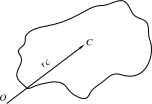
\includegraphics{figure/fig09.14}
    \caption{}
    \label{fig:09.14}
  \end{minipage}
  \begin{minipage}[b]{0.5\linewidth}
    \centering
    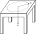
\includegraphics{figure/fig09.15}
    \caption{}
    \label{fig:09.15}
  \end{minipage}
\end{figure}
% 282.jpg

\clearpage
\exercise 一质量为$ m $的物体,绕一穿过光滑桌面上极小的圆孔的细
绳旋转(图\ref{fig:09.15})。开始时物体到中心的距离为$ r _ { 0 } $ ,旋转角速度为
$ \omega _ { 0 } $。若在$ t = 0 $ 时,开始以固定的速度$ v $拉绳子,于是物体到中心
的距离不断减小。求

(1) $ \omega \left( t \right) $ ;

(2)拉绳子的力$ F $。

\exercise 两个滑冰运动员,体重都是$ 60 $公斤,在两条相距$ 10 $米的平
直跑道上以$ 6.5 $米/秒的速率相向地匀速滑行。当他们之间的距离
恰好等于10米时,他们分别抓住一根$ 10 $米长的绳子的两端。若将
每个运动员看成一个质点,绳子质量略去不计。

(1)求他们抓住绳子前后相对于绳子中点的角动量。

(2)他们每人都用力往自己一边拉绳子,当他们之间距离为
$ 5.0 $米时,各自的速率是多少?

(3)计算每个运动员在减小他们之间距离时所做的功,并证
明这个功恰好等于他们动能的变化。

(4)求两人相距为$ 5.0 $米时,绳中之张力$ T $。

\exercise 两根均匀细杆,质量都是$ m $,长度都是$ l $,都以速率$ v $在垂
\begin{wrapfigure}[6]{r}{11em}
  \centering
  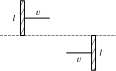
\includegraphics{figure/fig09.16}
  \caption{}
  \label{fig:09.16}
\end{wrapfigure}
直于长度方向平动,方向相反,如图
\ref{fig:09.15}所示。当它们相遇时,相邻两端
恰好相碰,而且粘接在一起形成一根
长为$ 2 l $的直杆。

(1)问碰撞后它们怎么运动?

(2)求碰撞后的角速度$ \omega $。

\exercise 如果地球的自转运动从现在的每$ 24 $小时一圈变成每$ 48 $小
时一圈,试估计地球与月球之间的距离将增为多少公里?已知地球
质量为$ M _ { E } = 6 \times 1 0 ^ { 2 4 } $公斤,地球半径$ R _ { E } = 6 4 0 0 $公里,月球质量$ M _ \text{ 月 }
  \approx 7 \times 1 0 ^ { 2 2 } $公斤,地月距离$ l \approx 3 . 8 \times 1 0 ^ { 5 } $公里,将月球视为质点。

\exercise 一个宇宙飞船环绕一行星作圆轨道运动,轨道半径为$ R _ 0 $,
% 283.jpg
飞船速率为$ v _ { 0 } $,突然点燃火箭,使飞船的速度从$ v _ { 0 } $变为$ \beta v _ { 0 } $,加
速度方向与速度方向同。

(1)求出用$ R _ 0, \beta $表示的新的轨道方程。证明当$ \beta < \sqrt { 2 } $时,
轨道是椭圆,总能为负;当$ \beta > \sqrt { 2 } $时,轨道为双曲线,总能为
正。

(2)在轨道为双曲线时,求出角度$ \alpha $的表达式(用$ \beta $表示$ \sin \alpha $或
$ \cos \alpha $),$ \alpha $为火箭点火时飞船速度方向与飞船逃逸时速度方向之间
的夹角;求出$ \beta = \sqrt { 3 } $时的$ \alpha $值。(提示:飞船逃逸时速度方向是
指飞船离行星为无穷远时的速度方向。)

\exercise 一个彗星在抛物线轨道上运行,此抛物线与地球的公转
轨道相交,两个交点在地球轨道直径的两端(设地球公转轨道为
圆)。

(1)若地球公转轨道的半径为$ R _ 0 $,地球公转速率为$ v _ { 0 } $,写出彗星的轨道方程。证明它的最大速率为$ 2 v _ { 0 } $。

(2)用开普勒第二定律证明彗星在地球轨道内的时间为
$ \dfrac { 2 } { 3 } \uppi $
年。

\exercise 已知地球半径$ R = 6 . 4 \times 1 0 ^ { 3 } $ 公里,密度为$ \rho = 5 . 5 $克/厘米\textsuperscript{3},
若地球为规则的球形,求地球自转的角动量。

\exercise 在静止的、均匀的、质量为$ M $、半径为$ R _ 1 $的水平大圆盘
上,站着一个质量为$ m $的人,圆盘可以无擦地绕通过圆盘中心
的竖直轴转动。当这个人开始顺着与圆盘周心、半径为$ R _ { 2 } $($ R _ { 2 } <
  R _ { 1 } $)的圆周等速率地走动时,若他相对于圆盘的速度为$ v $,问圆盘
将以多大的角速度$ \omega $旋转?

\exercise 在绕几何轴自由地旋转着的水平圆盘边上,站着一个质
量为$ m $的人。圆盘的半径为$ R $,转动惯量为$ I $,角速率为$ \omega = n $转/分。
若这人由盘边走到盘的中心,求圆盘角速度的变化和这个系统的
能量变化。
% 284.jpg

\exercise 如图\ref{fig:09.17},质量为$ m $、边长为$ a $的均匀正方形薄板,可以绕
着竖直轴$ O O ^ { \prime } $,自由地转动。当它静止时,有一质量为$ m $的小球以
速度$ v $沿水平方向垂直于板面撞在板的边上$ A $点。

(1)设碰撞是完全弹性的,碰撞后板和小球将如何运动?

(2)设碰撞是完全非弹性的,问小球与板共同的角速度$ \omega $为多
少?
\begin{figure}[h]
  \centering
  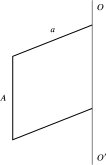
\includegraphics{figure/fig09.17}
  \caption{}
  \label{fig:09.17}
\end{figure}

\exercise 由于月一地之间有潮汐力,月亮会不断升高。当月一地相
距大致为多远时,月亮将会飞掉,不再随着地球公转了?

\end{exercises}
